%THIS IS AN EXAMPLE OF HOW YOU MIGHT INTRODUCE A CHAPTER WHICH HAS ALREADY BEEN PUBLISHED.
\cleartoevenpage
\pagestyle{empty}	%Use this to suppress the header from the preceding chapter.


\begin{table}[h]
	\begin{center}
	\begin{tabular}{|c|l|l|}
		\hline
		Contributor & Statement of contribution & \% \\
		\hline
		\textbf{Edward M. Barry}	    & writing of text 			& 70\\
										& proof-reading				& 60 \\
										& theoretical derivations 	& 70 \\
										& numerical calculations 	& 100\\
										& preparation of figures 	& 100 \\
										& initial concept			& 60 \\
		\hline
		Christopher T. DeGroot			& writing of text 			& 20\\
										& proof-reading				& 10 \\
										& supervision, guidance 	& 20\\
										& theoretical derivations 	& 10\\
										& preparation of figures 	& 20 \\
										& initial concept			& 10 \\
		\hline
		Shakil Ahmmed       			& writing of text 			& 20\\
										& proof-reading				& 10 \\
										& supervision, guidance 	& 20\\
										& theoretical derivations 	& 10\\
										& preparation of figures 	& 20 \\
										& initial concept			& 10 \\
		\hline
		Tim H\"{u}lsen		    		& writing of text 			& 10\\
										& proof-reading				& 30 \\
										& supervision, guidance 	& 80 \\
										& theoretical derivations 	& 20 \\
										& preparation of figures 	& 10 \\
										& initial concept			& 80 \\
		\hline
		Damien J. Batstone	    		& writing of text 			& 10\\
										& proof-reading				& 30 \\
										& supervision, guidance 	& 80 \\
										& theoretical derivations 	& 20 \\
										& preparation of figures 	& 10 \\
										& initial concept			& 80 \\
		\hline
	\end{tabular}
	\end{center}
\end{table}


%-------------------------------------------------------------------------------------------------------%
%-------------------------------------------------------------------------------------------------------%
%-------------------------------------------------------------------------------------------------------%
%-------------------------------------------------------------------------------------------------------%
%-------------------------------------------------------------------------------------------------------%
%-------------------------------------------------------------------------------------------------------%
%This is an internal chapter of the thesis.
%If you have a long title, you can supply an abbreviated version to print in the Table of Contents using the optional argument to the \chapter command.
\chapter[A multidimensional, phototrophic, continuum biofilm model]{A multidimensional, phototrophic, continuum biofilm model}
\label{chap:ch4}	%CREATE YOUR OWN LABEL.
\pagestyle{headings}

\section*{Abstract}

%-------------------------------------------------------------------------------------------------------%
%-------------------------------------------------------------------------------------------------------%
%-------------------------------------------------------------------------------------------------------%
\section{Introduction}
\label{sec:ch4_intro}
\subsection{Processes governing the biofilm lifecycle} 
Biofilms are communities of bacteria, algae, protozoa, fungi and other
microorganisms attached to a surface, and growing in an array of extracellular
polymeric substances \cite{loosdrecht2010}. % \cite{IWA book 2006 on biofilms}.
The lifecycle of a biofilm can be defined by the following processes:
\begin{enumerate}
    \item Initial attachment to the substratum surface
    \item Maturation of the biofilm
    \item Detachment of biomass
\end{enumerate}

The processes governing attachment are complex and varied. The physical properties of the solid substratum such as roughness, effective surface area,and hydrophobicity, play a role in the effectiveness of the attachment of microorganisms \cite{MarshallKevinC1990B/eb}. The ability of the surface to accept conditioning films (or protein rich coatings) and characteristics of the surrounding medium are also important factors for biofilm attachment \cite{donlan2002}. Hydrodynamic behaviour is also important for the attachment of cells. Until a certain critical shear stress where detachment occurs, cells have a higher probability of adhering to a surface the more times they come into contact with that substratum. This means that turbulent flow regimes are more conducive to biofilm attachment \cite{Rijnaarts1993}.

Planktonic organisms secrete chemical signals, however due to the dispersed distribution of suspended biomass, these signals have very little effect on genetic expression. Conversely, due to the dense distribution of organisms in the attached biofilm layer, maturation of the biofilm is influenced by quorum sensing, where the genetic expression of biofilm dwelling organisms is modified by chemical secretions of neighbouring organisms \cite{donlan2002}. The change in genetic expression leads to different behaviours in the biofilm. During biofilm formation, extracellular polymeric substances (EPS) are formed which lead to some benefits for the biofilm; \textit{a)} it acts as an adhesive for arriving organisms to the biofilm, \textit{b)} it forms protection from antimicrobial substances, leading to a resilience in the biofilm, and \textit{c)} it allows for transport of nutrients into the biofilm. As the biofilm continues to grow and expand, micro-niches form due to spatial variations such as nutrient diffusion and gas transfer limitations (anaerobes tend to aggregate near the biofilm-boundary layer interface, whereas anaerobes aggregate in oxygen poor environments. For photobiofilms, the consideration of the radiative distribution is also of interest as it's attenuation could also affect the spatial distribution of photoorganisms within a biofilm \cite{podola2017}. \\

The detachment of biomass occurs largely due to mechanical stresses. Erosion and sloughing occur depending on the nature of the flow field and boundary layer, and the shape and distribution of the biofilm itself. As detachment rates increase and balance growth rates, the biofilm remains in a quasi steady state \cite{xavier2005, storck2015}.

\subsection{Examples of beneficial and harmful biofilms}
It is important to understand the mechanisms of biofilm formation, whether the biofilm be beneficial or harmful. Examples of beneficial biofilms in process engineering applications include for the bioremediation of contaminated soils \cite{singh2006} and wastewater treatment applications where nutrients and impurities are removed from water streams through trickling filters or other engineered designs. Another application of interest in biotechnology is where biofilms aid in the harvesting of protein-rich bacteria, effectively short-cutting the need for expensive separation equipment associated with biomass thickening and dewatering \cite{Hulsen2016a}.

On the other hand, bad biofilms can also have such effects as reducing process equipment efficiency, being dangerous, harmful, or completely pernicious \cite{donlan2002}. Examples include the fouling on heat transfer and membrane equipment leading to a reduction in process performance \cite{mcdonogh1994199}, the formation of biofilms in food cultivation and preparation areas \cite{wirtanen2003}. The control of biofilms is vitally important in the health industry, as they present themselves as sources for inflammation, impaired healing, antimicrobial resistance, and patient death \cite{bryers2008}. As biofilm formation and growth can have significant positive or negative effects on society, the modelling of these systems is important in order to understand the details of the governing processes, therefore prevail in controlling such formation in practical applications. 


\subsection{Modelling of photobiofilms}
Biofilm models which capture the heterogeneities and spatio-temporal variations are \textit{de rigueur}. They are known as third generation models according to the IWA's task group on biofilm modelling. They build on the previous classes of biofilm modelling where steady-state, homogenous biofilms were defined in order to describe mass transport between biofilm and bulk flow (first generation) \cite{iwabiofilms}. Second generation models included updates to account for non-uniformities in the biofilm by describing microbial interactions. Third generation models can be described as either based on discrete agents, or as continuum models \cite{mattei2018}. Each approach has its own benefits and drawbacks.

\subsubsection{Discrete biofilm models}
There are two major discrete modelling approaches for biofilm formation: cellular automaton and agent based models. Cellular automaton models consist of discretising the spatial domain into discrete squares or cuboids for 2D or 3D models respectively. Each discrete element can be either occupied by a microbial cell, or a substance of interest, or can be empty. The cells are subjected to simple, discrete biological or physical operations \cite{mattei2018}. The operations, or rules, can include substrate diffusion, biokinetics expressions such as growth and decay, and attachment and detachment processes \cite{skoneczny2015}. Broadly accepted advantages of cellular automaton (CA) approaches are that the model setup oftentimes offers a simpler  development cycle as it is based on a series of discrete steps. In addition, the implementation of irregular boundary conditions is easier with this method \cite{pizzaro2001}, and the approach is known to be relatively simple to implement across multiple computing processors when compared to differential descriptions of states \cite{toffoli1987} . There are several disadvantages to the CA method, including the fact that conservation is not maintained under substrate uptake and growth processes, and the biofilm advances based on the availability of unoccupied cells. This means that dynamic growth and transformation processes closer to the substratum are often ignored \cite{mattei2018}. Additionally, as cells are effectively placeholders for physical information, the mesh cells are often of uniform phyiscal state. The accuracy is therefore dependent on the resolution of the meshed domain \cite{mattei2018}.

The other main method of discrete biofilm modelling is the agent based modelling (ABM) approach. This technique is similar to the CA approach insofar as it incorporates a set of rules that biomass follows. However, it differs in that the representation of biofilm species is as particulate matter, which can occupy any point in continuous spaces. Constraints due to the discretised CA lattice do not apply. Agent based models have been used to describe the interactions between multispecies particulates, including EPS formation and its effects on the the biofilm structure \cite{xavier2005a}. As the physical complexity of the modelled biofilm system increases, brute-force ABM simulations of complex systems often encounter computational limitations, limiting the spatial scale ofABMs. To overcome this limitation larger particles representing fractions of inert and active biomass has been presented. This type of model still follows ABM methods, with free-flowing particles, but the particles act as aggregate placeholders for physical information, similar to the CA methods \cite{picioreanu2004}. \\

Discrete approaches allow for the construction of complex models by building series of simple constraining rules. Model results often lead to a general idea of how the biofilm structure is formed, however agreement with experimental data is frequently case-specific \cite{mattei2018}. This is due to the description of the physical phenomena being based on a set of simple instructions with aspects of stochasticity. The order in which these instructions are executed can influence the results of the model, as well as the random nature of the discrete operations mean that results from identical initial conditions can differ significantly. Consequently, rigorous statistical analysis must be conducted in order to confirm the results from discrete models \cite{alpkvist2006}.

\subsubsection{Continuum-based biofilm models}
Continuum-based biofilm models can be classed into two main categories; one dimensional models (1D) and multidimensional models (2D for domains in $\mathbb{R}^2$-space and 3D for domains in $\mathbb{R}^3$-space respectively). Perhaps the most widely used 1D biofilm model is the AQUASIM implementation \cite{reichert1994} which builds upon the groundwork of \cite{wanner1986} \cite{wanner1986}. This model considers a multispecies competition and distribution within a biofilm. Included in the model are attachment and detachment processes, as well as considerations of mass transfer of soluble substrates within the porous structures. 1D biofilm model best lend themselves to particular cases: \textit{i)} in educational or demonstration settings, \textit{ii)} as part of broader or plant-wide models where mass exchange between biofilms and soluble substrates is to be quantified, but where computational requirements are to be used sparingly \cite{mattei2018}.

Multidimensional biofilm models are able to capture non-uniformities in the plan parallel to the surface substratum. Through this approach, one can explore the interactions between several species within a biofilm. Also, 2D and 3D approaches allow for analysis of time and space-dependent physical parameters and variables such as species and other particulate distribution, pressure gradients, and the interactions between soluble species and the porosity of the biofilm structure \cite{eberl2001}. Demonstrations in 1D and 3D test cases with varying symmetric and asymmetric boundary conditions were run, and the assessment of biofilm growth was found to agree well with experimental results. \cite{alpkvist2007}, (\cite{alpkvist2007}) also recognised the limitations associated with discrete models or 1D continuum models and thus proposed an extension to the Wanner-Gujer model as implemented in AQUASIM \cite{wanner1986}. The model linked a biomass volume fraction to Monod growth kinetics. The changes in volume fraction described changes in pressure which was the driver of biomass spreading. As the biofilm front represented a boundary and was dynamic, interface capturing was achieve with the level-set method, which allows for the reconstruction of the biomass front from a differential distance function. 2D and 3D simulations were carried out, and the results showed the formation of microbial niches due to substrate gradients. This model represents one of the first examples of a mathematically rigorous approach being taken to biofilm modelling.

\subsubsection{Photobiofilm models}
As the field of study of photobioreactors is in its infancy, the benefits of photobiofilm reactors have seldom been discussed. It has been indentified that the harvesting, thickening and dewatering costs associated with phototrophic processes could be reduced if growth by attachment was the dominant growth mode in photobioreactors  \cite{Hulsen2016a}. Purple phototrophic bacteria (PPB) are known to form heterogeneous, somewhat stratified biofilm structures in benthic zones of aquatic environments \cite{Overmann2006}, however algal biomass has proven more difficult to engineer into biofilm formations. A recent attempt to foster a mycoalgal biofilm proved to be more effective than in the axenic cultures \cite{rajendran2016}, but for applications such as waste treatment, one doesn't have the privilege of being able to select specific co-cultures. That said, whatever the application of photobiofilm systems, that elucidation of the process kinetics coupled with biofilm development is required for a deeper understanding, especially with respect the coupling with the radiative field.

With regards to phototrophic biofilm modelling, only two examples exist prior to this work. The first phototrophic biofilm (PBF) model was proposed as a two dimensional application to a porous susbstrate photobioreactor (PSBR) \cite{murphy2014}. The model looked at the productivity of \textit{Anabaena variabilis}, a cyanobacterium, through substrate transport, photon delivery, and growth processes. There was good agreement between numerical simulations and experimental results with respect to biomass productivity over a range of thicknesses between \SI{35}{\micro\metre} and \SI{45}{\micro\metre}. This model focused on a pure culture of cyanobacteria, and the evolution of biofilm structure was not explored in this scope. Additionally, variations in soluble substrate concentrations into the biofilm towards the surface substratum were not presented. \\

The second study focused on a 1D application of a PBSR \cite{Li2016}. This model extended the previously mentioned study with respect to the substrate gradients perpendicular to the biofilm surface substratum. The radiative transfer equation was used to simulate the light delivery to the biofilm concluded that phase in-scattering and pigment adaptation were important considerations. The advection of the biofilm front was by treating the biomass length as a discrete quantity, either consuming or releasing discrete elements at each simulated time step. \\

The proposed model in this paper differs from the previous PBF examples in the following aspects:
\begin{enumerate}
\item Biofilm models should be developed for implementation in all spatial dimensions. Decisions to simplify the model should be made by the user at implementation. Presented here is a multidimensional phototrophic biofilm model.
\item The evolving structure of the biofilm must be captured. The advancement of the biofilm front is coupled to biomass growth and decay processes. The interface between biofilm and liquid is captured by a conservative, coupled volume-of-fluid (VoF) and level-set method.
\item Biofilms are heterogeneous in nature. Scope must be made to model multispecies biofilm evolution. As such, presented here is a multidimensional,  multispecies, dynamically structured phototrophic biofilm model.
\end{enumerate}

In addition to these three points of novelty, the biofilm model has been implemented in OpenFOAM, a computational fluid dynamics (CFD) finite volume method (FVM) framework. This package is a collection of C++ libraries which allow for the resolution of continuum mechanics problems. The model extends on previous work by the authors \cite{Puyol2017}. The global purpose of this study is to explain the physical phenomena occurring within biofilms so that subsequent studies can progress the work for design or prediction purposes.

%As biofilms are spatially heterogeneous structures, both spatial and temporal variations must be considered in order to describe the physical phenomena. Biofilm models can be divided into three main classes: \textit{i)} one-dimensional models capable of including mass transfer, reaction/diffusion, and detachment processes \cite{horn2014}, \textit{ii)} multidimensional discrete biofilm models such as cellular automata and agent based methods \cite{wang2010}, and \textit{iii)} continuum models including computational fluid dynamics (CFD) approaches \cite{alpkvist2007, duddu2009, cunault2015}. Despite the vast suite of modelling approaches and examples existing within the literature, there have been few studies which defining biofilm behaviour in phototrophic systems, where the spatially varying nature of the radiative field could be an important factor in the heterogeneous formation of biofilms. \\

%Representing biomass as continua can be advantageous. Firstly, the currency of process engineering modelling is differential balance equations. Continuum modelling is therefore a common language for communication of model development and results, and additionally, conservation of differential states can be ensured. In contrast to discrete modelling methods, deterministic solutions can be obtained for continuum-based models \cite{mattei2018}. Difficulties can arise when modelling continuum-based biofilms. The frequently abrupt density jumps across liquid/solid boundaries can lead to numerical instabilities. The coupling of the non-linear transport equations with growth kinetics can also be problematic. Additionally, solving state equations with vastly different time constants (and order of 10s of seconds for fluid flow in a reactor, to hours or days for biomass growth and decay expressions) can make the resolution of the time discretisation difficult. Differential algebraic equations, or appropriate time discretion algorithms for stiff systems of differential equations can overcome this barrier. Computational fluid dynamics (CFD) packages can assist with some of the numerical problems and the mathematical formulation difficulties associated with continuum models.


% \begin{itemize}
% \item Biofilms are communities of microorganisms, EPS matrices and inert substances living together
% \item There are extrinsic properties leading to their growth:
% \begin{itemize}
% \item fluid flows
% \item irradiance
% \item presence of nutrients
% \item presence or absence of other microorganisms
% \item shear rates
% \item reactor geometry and operating conditions (implicitly)
% \end{itemize}
% \end{itemize}


%Whether biofilms are desired or not, a continuum based photobiofilm model has been created in order to encapsulate the important physical conditions of systems to achieve the desired ends. 



%\begin{instructional}
%Add your text here. Use \verb|\cite| to add citation labels. Reference sections, tables, and figures using \verb|\ref|. Use \verb|\eqref| for equations. The `section' symbol $\S$ is obtained using \verb|$\S$|. Figures and other floats are added using their respective environments. Use \verb|\longtable| to split tables over page.
%\end{instructional}


%%%% PROBLEM DESCRIPTION
\newpage
\section{Problem description}
\label{S:problem_description}
The modelling approach is concerned with the description of a phototrophic biofilm system consisting of purple phototrophic bacteria (PPB). The model description for this system has been previously described \cite{Puyol2017}, however this did not account for spatial variations, and by extension, biofilm formation was not considered. The phototrophic biofilm grows attached to a surface substratum. Above the biofilm is a body of nutrient-rich liquid. Incident photons of wavelength 850 \si{\nano \metre} are irradiated from either \si{\Gamma_0} or \si{\Gamma_3} into the domain \si{\Omega}, as shown in Fig. \ref{fig:2d_above}. The initial thickness of the biofilm is \SI{50}{\micro \metre} with uniformly distributed solid species. The factor of incident irradiance is also explored, with three different irradiance levels of \SI{10}{\watt \metre ^2}, \SI{30}{\watt \metre ^2}, and \SI{100}{\watt \metre ^2} being simulated from the surface substratum. Incident irradiance in all cases is assumed uniform and diffuse across the whole boundary.


% The phototrophic biofilm (PBF) model based on purple phototrophic bacteria is an extension of the models presented previously \cite{Puyol2017} (\textbf{include my model}). Biofilm treatment extends work previously carried out by \cite{alpkvist2007}, \cite{alpkvist2007}. The important physical processes identified are as follows:
% \begin{itemize}
%     \item Coupled volume of fluid and level set for capturing of the biofilm/liquid interface.
%     \item Radiative transfer coupled to the growth of the biokinetics.
%     \item Biokinetics equations coupled to the radiative transfer equation (RTE) and the biofilm advection terms.
%     \item Development of a biofilm front velocity based on the evolution of pressure due to solid species growth within the biofilm.
% \end{itemize}


\begin{figure}[htpb]
    \centering
    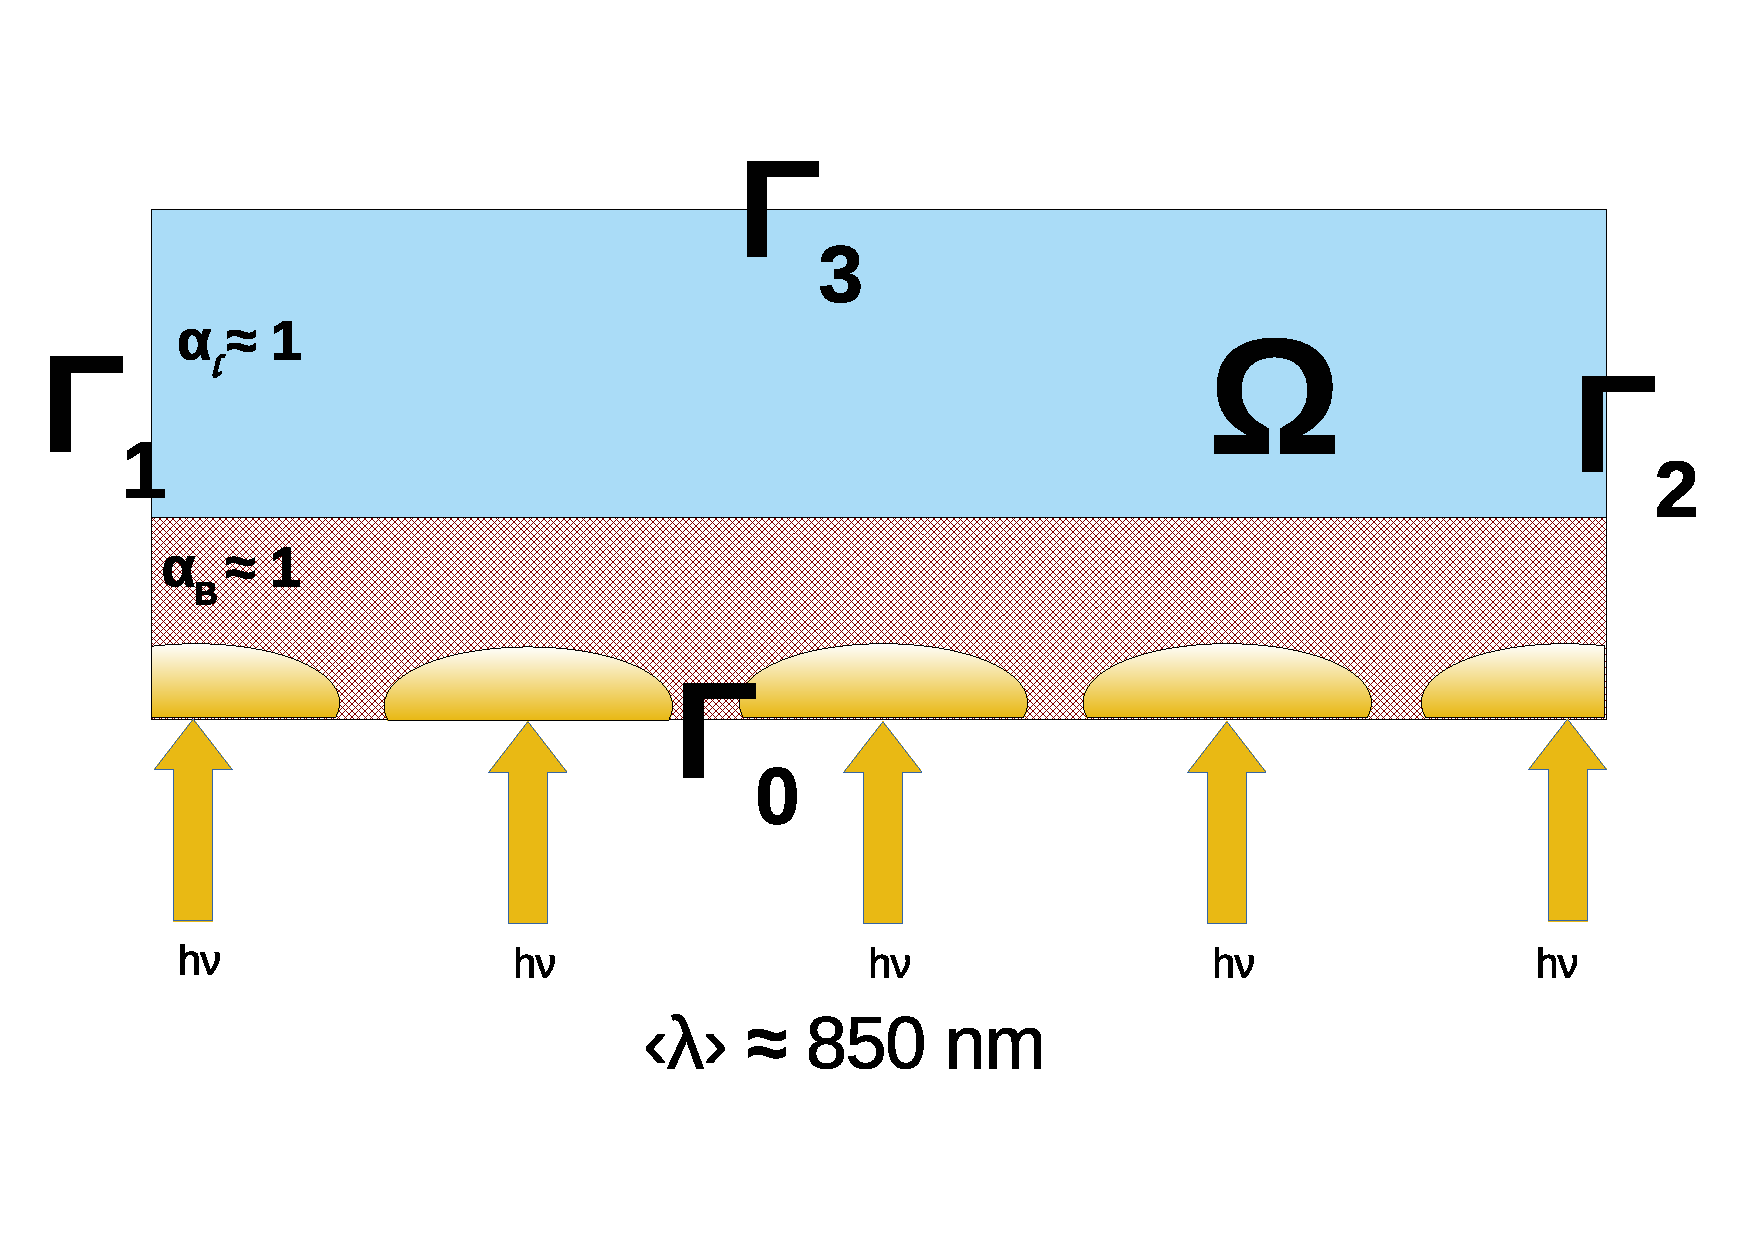
\includegraphics[scale=0.5]{Images/Chap4/prob_diagram_below.pdf}
    \caption{Two-dimensional representation of the simulation domain for the case of a bottom-irradiated biofilm. Boundaries \si{\Gamma_4} and \si{\Gamma_5} are out of, and into the page respectively, and take the same boundary conditions as boundaries \si{\Gamma_1} and \si{\Gamma_2}. The irradiance source (\si{h \nu}) is in fact uniform and diffuse across the whole boundary. Subscripts relating to \si{\alpha}, namely \textbf{l} and \textbf{B} correspond to liquid phase fraction, and biofilm phase fraction respectively.} 
    \label{fig:2d_above}
\end{figure}


%%%%%%%%%%%%% MATHEMATICAL FORMULATION

\newpage
\section{Mathematical formulation}
\label{S:formulation}
\subsection{Radiative transfer}
The general form of the radiative transfer equation (RTE) has been adapted to phototrophic systems \textbf{cite me} \cite{Kong2014}, and includes the dependency on the concentration of solid species and water. The black body radiation term has been omitted from this equation due to minimal influence on the system energy balance (Eq. \ref{eq:rteSimplified}). 

\begin{equation}
\frac{dI_\lambda (\textbf{r}, \textbf{s})}{ds} \, = \, - \sum_{j} [E_{\lambda,j} X_j] I_\lambda (\textbf{r}, \textbf{s})\, +\, \frac{\sigma_{\lambda, s, j}}{4 \pi} \int_{4 \pi} I_\lambda (\textbf{r}, \textbf{s}^\prime) \Phi_\lambda(\textbf{s}, \textbf{s}^\prime) d\Omega^\prime
    \end{equation}

where $I_\lambda$ is the spectral irradiance for a given wavelength, \textbf{r} is the position vector of a radiative ray, \textbf{s} is the direction vector of the ray, and s is the path length. The first term on the right hand side is the extinction term, with $E_{\lambda, j}$ being the specific extinction coefficient (the combination of scattering and absorption components) for participating species $X_j$. The second term on the right hand side is associated with in-scattering, where $\sigma_{\lambda, s, j}$ is the scattering coefficient, and $\Phi_\lambda$ is the wavelength scattering function from path \textbf{s} to scattered direction $\textbf{s}^\prime$ through solid angle $d\Omega$. The phase scattering function, $\Phi_\lambda$ for this model is the Schlick function (Eq. \ref{eq:schlick}), which is appropriate for optically thick media \cite{Jarosz2008}. 

\begin{equation}
\Phi_s(k, \theta) = \frac{1 \, -\,  k^2}{4\pi (1\, +\,k\, cos(\theta))^2 }
\end{equation}

where parameter $k$ takes values between -1.0 and 1.0 included, with negative or positive values corresponding to back-scattering and forward scattering respectively. A value of 0 means scattering is isotropic. The parameter $k$ represents the average cosine of the scattered angles. The angle $\theta$ is that made by the previous path and scattered path of a ray.

\subsection{Consumption and release of soluble substrates}
Soluble substrates exist in both the volume of liquid, and the biofilm volume. Their growth and release expressions (hydrolysis of biodegradable particulate organic matter) have been previously described \cite{Puyol2017}. The soluble substrates considered in this study are readily biodegradable soluble organics expressed in chemical oxygen demand (COD), acetic acid (COD), hydrogen (COD), inorganic carbon (C), inorganic nitrogen (N), inorganic phosphorus (P) and soluble inert material (COD). The general form for the soluble balance equation is expressed in Eq. \ref{eq:solubles}.

\begin{equation}
\label{eq:solubles}
\frac{\partial S_i}{\partial t} = \mathcal{D}_i\nabla^2 S_i + r_{i}
\end{equation}

where $S_i$ is the soluble species $i$, $\mathcal{D}_i$ is the diffusion coefficient of species $i$, and $r_i$ is the corresponding consumption/release equation \cite{Puyol2017}. 

\subsection{Growth of particulate matter}
The growth of particulate matter forms the biofilm structure and influences the pressure equation which influences advection of the biofilm front. The particulate species included in this study are PPB, slowly biodegradable particulate organics, and inert particulate organic matter. Similarly to \cite{alpkvist2007}, replace $X_i$, the concentration of particulate species $i$ with $\rho^*\theta_i$ where $\rho^*$ is the density of particulate species, assumed constant for each species, and $\theta_i$ is the volume fraction of species $i$. The growth terms for the particulate balance equations (Eq.~\ref{eq:particulates}) have been previously defined \cite{Puyol2017}.


\begin{equation}
    \label{eq:particulates}
    \frac{\partial \theta_i}{\partial t} = \lambda \nabla p \cdot \nabla \theta_i + \frac{g_i}{\rho^*} - \theta_i \sum_{i=1}^{N_{\theta_i}}\frac{g_i}{\rho^*}
\end{equation}

where 


\subsection{Pressure term}
The pressure term drives the advection of the biofilm front. It depends on the growth or decay of the solid species. All terms in this equation (Eq.~\ref{eq:pressure}) have already been defined. 

\begin{equation}
    \label{eq:pressure}
    -\nabla^2p = \sum_{i=1}^{N_{\theta_i}} \frac{g_i}{\rho^*}
\end{equation}


\subsection{Boundary and initial conditions}
These need to be included once debugging has finished.


%%%%%%%%%%%%% Numerical Treatment
\section{Numerical Treatment}






%%%%%%%%%%%%%%%%% Implementation
\section{Implementation}
















%%%%%%%%%%%%%%%%%%%%%%%% DISCUSSION
\section{Discussion}



















%%%%%%%%%%%%%%%%%%% CONCLUSIONS
\section{Conclusions}